../cictikz/src/cictikz/data/tex/cictikz_preamble.tex

% Both sensors measured against a Voetsch climate chamber from 5 to
% 70 degrees C. (a) The output rate against the chamber's own probe: a
% PTAT current into a fixed capacitor should give a rate proportional to
% absolute temperature, and it does. GR06 is plotted on the right axis
% scale, six times lower, because it is read once per reset rather than
% free-running. (b) What is left after the best straight line, expressed
% in kelvin through each sensor's own slope. Neither is limited by
% linearity: GR07's 1.6 K is dominated by the 4.75 K staircase from
% re-timing its output on the project clock.
%
% Generated by py/tikzplot.py. Edit the script in ex/ that
% produced it and re-run that, not this file.

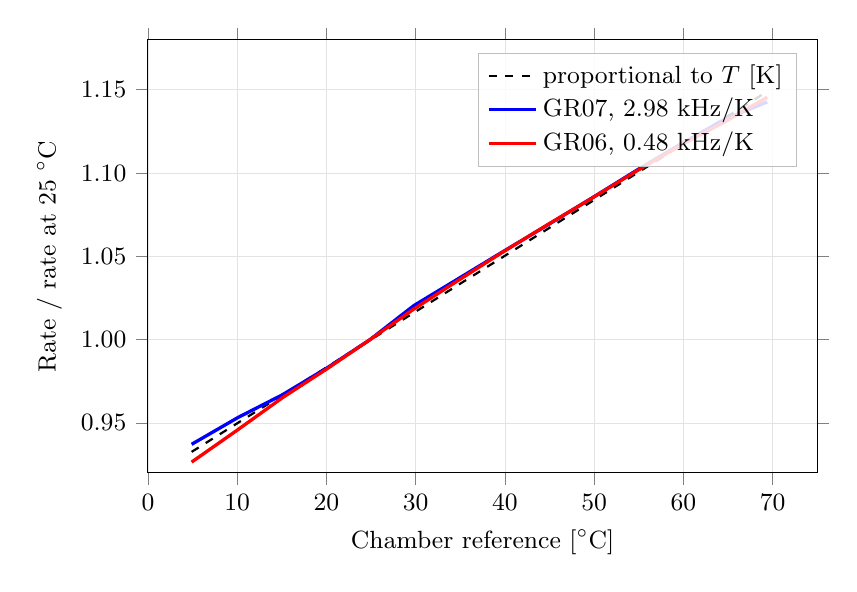
\begin{tikzpicture}[thick]

\begin{axis}[
  width=8.5cm,
  height=5.5cm,
  scale only axis,
  grid=both,
  grid style={gray!22, very thin},
  tick align=outside,
  tick label style={font=\small},
  label style={font=\small},
  title style={font=\small, yshift=-1mm},
  legend cell align=left,
  legend style={font=\small, draw=gray!50, fill=white, fill opacity=0.85, text opacity=1},
  xlabel={Chamber reference [$^\circ$C]},
  ylabel={Rate / rate at 25 $^\circ$C},
  scaled y ticks=false,
  yticklabel style={/pgf/number format/fixed, /pgf/number format/zerofill, /pgf/number format/precision=2},
  xmin=0,
  xmax=75,
  ymin=0.92,
  ymax=1.18,
  legend pos=north east
]
\addplot[black, thick, dashed, mark=none] coordinates {(4.9,0.93258) (10.1,0.95003) (15.1,0.9668) (20.1,0.98357) (24.9,0.99966) (29.8,1.0161) (34.8,1.0329) (39.7,1.0493) (44.7,1.0661) (49.7,1.0828) (54.7,1.0996) (59.7,1.1164) (64.7,1.1332) (69.4,1.1489)};
\addlegendentry{proportional to $T$ [K]}
\addplot[blue, very thick, mark=none] coordinates {(4.9,0.93712) (10.1,0.95323) (15.1,0.96694) (20.1,0.98306) (24.9,1) (29.8,1.0204) (34.8,1.0366) (39.7,1.0525) (44.7,1.0685) (49.7,1.0848) (54.7,1.1014) (59.7,1.1173) (64.7,1.1324) (69.4,1.1427)};
\addlegendentry{GR07, 2.98 kHz/K}
\addplot[red, very thick, mark=none] coordinates {(4.9,0.92644) (10.1,0.94596) (15.1,0.96518) (20.1,0.98256) (24.9,1) (29.8,1.0183) (34.8,1.0356) (39.7,1.0523) (44.7,1.0687) (49.7,1.0847) (54.7,1.101) (59.7,1.1167) (64.7,1.1309) (69.4,1.1455)};
\addlegendentry{GR06, 0.48 kHz/K}
\end{axis}

\end{tikzpicture}
\end{document}
